\documentclass{llncs}

%\usepackage{makeidx}  % allows for indexgeneration
\usepackage{amsfonts}
\usepackage{amssymb,amsmath}
\usepackage{algorithm}
\usepackage{algpseudocode}
\usepackage{graphicx}
\usepackage{multicol}
\usepackage{subfigure}

\newcommand{\spc}{\phantom{a}}

\begin{document}

%\frontmatter          % for the preliminaries

\pagestyle{headings}  % switches on printing of running heads

\title{A shuffled complex evolution algorithm for
the multidimensional knapsack problem}

\author{
   Marcos Daniel Valad\~ao Baroni\thanks{Research supported by Funda\c c\~ao de Amparo \`a Pesquisa do Esp\'irito Santo.}
   \and
   Fl\'avio Miguel Varej\~ao
}

\institute{Universidade Federal do Esp\'irito Santo,\\
Av. Fernando Ferrari, 514, Goiabeiras, Vit\'oria, ES, Brazil\\
\texttt{http://ninfa.inf.ufes.br/}
}

\maketitle              % typeset the title of the contribution

\begin{abstract}
This work addresses the application of
a population based evolutionary algorithm
called shuffled complex evolution (SCE) in the multidimensional knapsack
problem.
The SCE regards a natural evolution happening simultaneously in independent communities.
The performance of the SCE algorithm is verified through computational experiments
using well-known problems from literature and randomly generated problem as well.
The SCE proved to be very effective in finding good solutions demanding a
very small amount of processing time.
\keywords{ Multidimensional knapsack problem, Meta-heuristics, Artificial Intelligence}
\end{abstract}

\section{Introduction}
\label{sec:intro}

The multidimensional knapsack problem (MKP) is a strongly NP-hard combinatorial
optimization problem which can be viewed as a resource allocation problem and
defined as follows:

\begin{align}
  \text{maximize} & \sum_{j=1}^n p_j x_j \\
  \text{subject to} & \sum_{j=1}^n w_{ij} x_j \leqslant c_i \quad i \in \{1, \ldots, m\}\\
   & x_j \in \{0, 1\}, \quad j \in \{1, \ldots, n\}.
\end{align}

% Define the MKP
The problem can be interpreted as a set of $n$ items with profits $p_j$
and a set of $m$ resources with capacities $c_i$.
Each item $j$ consumes an amount $w_{ij}$ from each resource $i$, if selected.
The objective is to select a subset of items with maximum total profit,
not exceeding the defined resource capacities.
The decision variable $x_j$ indicates if $j$-th item is selected.
It is considered an integer programming problem (IP) since its variables $x_i$
are restricted to be integers.

The multidimensional knapsack problem can be applied on budget planning 
scenarios and project selections~\cite{mcmillan1973resource},
cutting stock problems~\cite{Gilmore-Gomory-1966}, loading problems~\cite{Shih-1979},
allocation of processors and databases in distributed computer programs~\cite{Gavish-Pirckul-1982}.

The problem is a generalization of the well-known knapsack problem (KP) in which
$m = 1$.
However it is a NP-hard problem significantly harder to solve in practice than the KP.
%Despite the existence of a fully polynomial approximation scheme (FPAS) for the KP,
%finding a FPAS for the MKP is NP-hard for $m \geqslant 2$~\cite{magazine1984note}.
Due its simple definition but challenging difficulty of solving, the MKP is often used to
to verify the efficiency of novel metaheuristics.

Its well known that the hardness of a NP-hard problem grows exponentially over
its size.
Thereupon, a suitable approach for tackling NP-hard problems is to reduce their size
through some variable fixing procedure.
Despite not guaranteeing optimality of the solution, an efficient variable
fixing procedure may provide near optimal solutions through a small computational effort.

%A metaheuristic is a set of concepts that can be used to define heuristic methods
%that can be applied to a wide set of different problems.
%In other words, a metaheuristic can be seen as a general algorithmic framework which can be applied to
%different optimization problems with relatively few modifications to make them adapted to a specific problem.”

The SCE is a metaheuristic proposed by Duan in \cite{duan1992effective}
which combines the ideas of a controlled random search with the concepts
of competitive evolution and shuffling.
The SCE algorithm has been successfully used to solve several problems
like flow shop scheduling~\cite{zhao2014shuffled}, project management~\cite{elbeltagi2007modified}
and MKP~\cite{baroni2015shuffled}.

This work addresses the development of an hybrid heuristic using an
efficient variable fixing procedure and the SCE metaheuristic, as an improvement
proposal for the work in \cite{baroni2015shuffled}

The reminder of the paper is organized as follows:
Section~\ref{sec:core} defines the core concept for the MKP and its application
in the problem reduction.
Section~\ref{sec:sce} presents the shuffled complex evolution algorithm
and proposes its application on the MKP.
Section~\ref{sec:exp} comprises several computational experiments over well-known
instances from literature.
In section~\ref{sec:conc} we make our concluding remarks about the developed
methods and the experimental results.



\section{The shuffled complex evolution for the MKP}
\label{sec:sce}
The {\bf shuffled complex evolution} (SCE) \cite{duan1992effective}
is a population
based evolutionary optimization algorithm that regards a natural 
evolution happening simultaneously in $N$ independent communities (or {\bf complexes}).

Initialy $N*M$ individuals are randomly taken from the feasible solution space and
sorted according to their fitness.
Subsequently a {\bf shuffling} process places the \nth{1} in the first complex,
the \nth{2} in second complex, individual N\ts{th} goes to N\ts{th} complex,
individual $M+1$ goes back to the first complex, etc.
\vspace*{-20pt}
\begin{center}
\noindent\begin{tabular}{@{\hspace{0.0em}}c@{\hspace{1.0em}}c@{\hspace{0.0em}}}
\hspace{-3mm}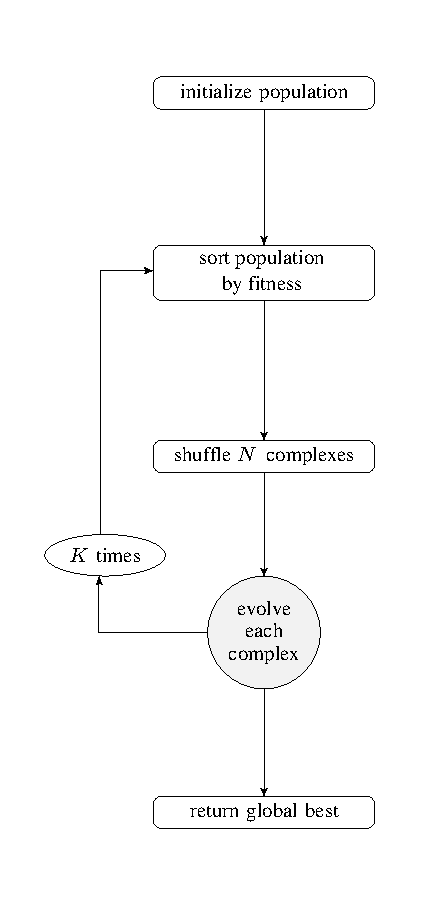
\includegraphics[width=0.46\linewidth]{imgs/flow1a} &
\hspace{-3mm}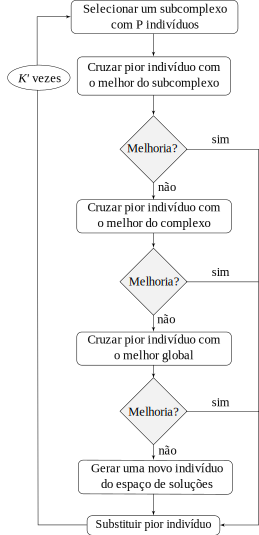
\includegraphics[width=0.46\linewidth]{imgs/flow2} \\
{\scriptsize The SCE algorithm.} & {\scriptsize Evolving stage.}
\end{tabular}
\end{center}
The next step after shuffling the complexes is to evolve each each of then through
a fixed amount of {\it (a)} $K'$ steps.
In each step {\it (b)} a {\bf subcomplex} of $P$ individuals is selected from the
complex, prioritizing those with better fitness.

The worst individual from the  subcomplex is identified to
be replaced by a new one generated by {\it (c)} its crossing 
with best individual of the subcomplex.

If the new solution has not improved {\it (d)} the best individual
of the {\bf complex} is considered for crossing and latter the {\it (e)} best one  
of whole {\bf population}.
If all the crossing steps couldn't improve the worst individual,
it is {\it (f)} replaced by a {\bf new random} solution.


\section{Computational experiments}
\label{sec:exp}

\subsection{Experimental Setup}
%\subsubsection{Computational Environment}
All experiments were run in Intel Core i5-2310 CPU @ 2.90GHz machines
with 8GB of RAM memory running Linux Mint 13 64 bits.  To facilitate the job distribution we have used the HTCondor framework.

%\subsubsection{Parameters}
The GALP algorithm has no settable parameters, the TSLP algorithm on the other hand,
has 3 parameters: the number of iterations of the Tabu Search algorithm (10000),
the size of the tabu list (1000) and the number of random neighbors per iteration
($n_{tabu}$ = 500).
The parameters were set up by empirically experimenting several different combinations.

%\subsubsection{Implementation}
To solve the integer programming problems we have used the GLPK LP/MIP solver \cite{GLPK},
version 4.43. We have implemented the heuristics using the Java programming language and
executed/compiled the codes using the Java(TM) SE Runtime Environment (build 1.7.0\_10-b18).
All implementations are available at \url{http://ninfa.inf.ufes.br/ICTAI2013/impl.zip}. 

%\subsection{Instance Generator}
To create the instances for our analysis we have implemented a random instance generator,
with parameters inspired by real-world actions given by the local EDCO.
The generator was implemented in the Python programming language and its implementation 
and random instances are available at \url{http://ninfa.inf.ufes.br/ICTAI2013/gen.zip}.

\subsection{Time Analysis}

\subsubsection{The Impact of Correlation}                      
It has been demonstrated the classical  Knapsack Problem is pseudo-polynomial
in the size of the input \cite{garey1978} and it is a established
fact that a weak correlation among weight and value greatly reduces the difficulty of the instances \cite{david2005}.
Literature on the knapsack problem states that the difficult problems are the ones that exhibit 
a strong correlation between the value of the item and its weight.

To test if this phenomena also happens in our problem, we have tested the values $[0.0, 0.1, 1.0]$ for $\alpha$,
the parameter that controls the correlation of the value of the action in respect to its cost, 
in a number of problem sizes. When $\alpha$ is 0,
there is a strong correlation between the cost of the action and its electricity return, that is,
the more expensive the action, the more effective it is. When $\alpha$ is 1 there is no correlation
between the value of the actions and its effectiveness. When $\alpha$ is 0.1, there is a weak correlation between cost and value.
The $\alpha$ values of 0.0, 0.1 and 1.0 are equivalent to the following classes of problems defined by \cite{david2005} (respectively): 
\textit{subset sum instances, weakly correlated instances and uncorrelated instances.}

To measure running times we have generated instances for each considered $\alpha$, varying both the amount of years and actions
in the interval $[5,15]$. For each triple defined by the value of $\alpha$, the number of years and actions,
we have generated 10 instances and measured their running time to find the exact solution. 
We have observed that the variance of the running times to solve these 10 instances was too large
for the mean to be significative, so we have adopted a alternative strategy to compare problem sizes
and $\alpha$:
we assume that running times of more than one hour are prohibitive for our application, since
EDCOs usually test several portfolios to make their investment decision. So we consider that
these instances failed to find the solution in practical times.

Figures~\ref{fig:time1} to~\ref{fig:time3} display the amount of instances that successfully executed in less than one hour,
given a value of $\alpha$. For each cell of the figure the exact algorithm was run 10 times using random instances of the problem.
The closer to black, the greater the amount of successful runs. 
From the figures it is clear that the bigger the problem the more likely it is that it will take more than one hour to execute, 
since cells closer to $(15,15)$ tend to be closer to white.
Also, it may be observed that the more
correlated the cost is with the profit (the smaller the $\alpha$),
the harder the problems seems to be, as predicted by the literature.

%\begin{figure}
%  \begin{subfigure}{0.45\textwidth}
%    \includegraphics[scale=0.5, trim=0.75cm 0cm 0 2cm, clip=true]{imgs/very_hard.pdf}
%    \caption{Strong correlation between cost and profit.}
%    \label{fig:time1}
%  \end{subfigure}
%  \begin{subfigure}{0.45\textwidth}
%    \includegraphics[scale=0.5, trim=0.75cm 0cm 0 2cm, clip=true]{imgs/hard.pdf}
%    \caption{Weak correlation between cost and profit. \\ $\,$ }
%    \label{fig:time2}
%  \end{subfigure}
%  \begin{subfigure}{0.45\textwidth}
%    \includegraphics[scale=0.5, trim=0.75cm 0cm 0 2cm, clip=true]{imgs/easy.pdf}
%    \caption{No correlation between cost and profit.}
%    \label{fig:time3}
%  \end{subfigure}
%\end{figure}

\begin{figure}[H]
  \begin{subfigure}{0.45\textwidth}
    \includegraphics[scale=0.5, trim=0.75cm 0cm 0 2cm, clip=true]{imgs/very_hard.pdf}
    \caption{Strong correlation between cost and profit.}
    \label{fig:time1}
  \end{subfigure}
  \begin{subfigure}{0.45\textwidth}
    \includegraphics[scale=0.5, trim=0.75cm 0cm 0 2cm, clip=true]{imgs/hard.pdf}
    \caption{Weak correlation between cost and profit. \\ $\,$ }
    \label{fig:time2}
  \end{subfigure}
  \begin{subfigure}{0.45\textwidth}
    \includegraphics[scale=0.5, trim=0.75cm 0cm 0 2cm, clip=true]{imgs/easy.pdf}
    \caption{No correlation between cost and profit.}
    \label{fig:time3}
  \end{subfigure}
  \caption{Number of aborted instances for exact approach.}
\end{figure}

\subsection{Solution Analysis - Easy Instances}

In this subsection we compare the solution quality of the implemented heuristics
in the set of easy instances, there is, the instances in which the exact algorithm
found the optimal solution in less than one hour. We have also limited the running time
of the heuristics in one hour.

Figures~\ref{fig:mh1_1} to \ref{fig:mh2_3} display the average ratio between the optimal solution (when available) 
and the solution found by the heuristics. 
Small relative ratios are darker than large differences.
A ratio of 1 means that the heuristic has found a solution with the same quality
than the exact algorithm.
When no solution was found by the exact approach in less than one hour for 
a tripe $(\alpha, years, actions)$, we display the value ``$na$'' in
the corresponding cell.

Figures~\ref{fig:mh1_1} to \ref{fig:mh2_3} show that all heuristics managed
to find very close solutions to the exact (less than 1\% difference).
Also, the paler aspect of the TSLP figures (specially when $\alpha=0.0$) suggests that
it managed to beat the GALP algorithm considering solution quality.
In fact, considering only these easier problem sizes, the paired Wilcoxon signed-rank test \cite{japkowicz2011evaluating} rejects the null hypothesis
that the algorithms are the same with a $p$-value of less than $10^{-11}$.

\begin{figure}
  \begin{subfigure}{0.45\textwidth}
    %\centering
    \includegraphics[scale=0.5, trim=0.75cm 0.55cm 0 2cm, clip=true]{imgs/comp_very_hard.pdf}
    \caption{Solution by GALP for $\alpha=0.0$.}
    \label{fig:mh1_1}
  \end{subfigure}
  \begin{subfigure}{0.45\textwidth}
    %\centering
    \includegraphics[scale=0.5, trim=0.75cm 0.55cm 0 2cm, clip=true]{imgs/comp_very_hard_ts.pdf}
    \caption{Solution by TSLP for $\alpha=0.0$.}
    \label{fig:mh2_1}
  \end{subfigure} 
  \begin{subfigure}{0.45\textwidth}
    \includegraphics[scale=0.5, trim=0.75cm 0.55cm 0 2cm, clip=true]{imgs/comp_hard.pdf}
    \caption{Solution by GALP for $\alpha=0.1$.}
    \label{fig:mh1_2}
  \end{subfigure}
  \begin{subfigure}{0.45\textwidth}
    \includegraphics[scale=0.5, trim=0.75cm 0.55cm 0 2cm, clip=true]{imgs/comp_hard_ts.pdf}
    \caption{Solution by TSLP for $\alpha=0.1$.}
    \label{fig:mh2_2}
  \end{subfigure}
  \begin{subfigure}{0.45\textwidth}
    \includegraphics[scale=0.5, trim=0.75cm 0.55cm 0 2cm, clip=true]{imgs/comp_easy.pdf}
    \caption{Solution by GALP for $\alpha=1.0$.}
    \label{fig:mh1_3}
  \end{subfigure}
  \hspace{1cm}
  \begin{subfigure}{0.45\textwidth}
    \includegraphics[scale=0.5, trim=0.75cm 0.55cm 0 2cm, clip=true]{imgs/comp_easy_ts.pdf}
    \caption{Solution by TSLP for $\alpha=1.0$.}
    \label{fig:mh2_3}
  \end{subfigure}
  \caption{Comparison between the optimal solution (when available) 
  and the solution by heuristic methods.}
\end{figure}

\begin{figure}
  \begin{subfigure}{0.45\textwidth}
    \centering
    \includegraphics[scale=0.5, trim=0.75cm 0cm 0 2cm, clip=true]{imgs/comp_very_hard_sg_ts.pdf}
    \caption{$\alpha=0.0$.}
    \label{fig:comp_1}
  \end{subfigure}
  \hspace{1cm}
  \begin{subfigure}{0.45\textwidth}
    \centering
    \includegraphics[scale=0.5, trim=0.75cm 0cm 0 2cm, clip=true]{imgs/comp_easy_sg_ts.pdf}
    \caption{$\alpha=1.0$.}
    \label{fig:comp_3}
  \end{subfigure}
\end{figure}

\subsection{Solution Analysis - All Instances}

In this subsection we compare the behavior of the metaheuristics in respect to one another
considering all instances. We cannot compare the results with the optimal solution since they are unknown for the harder instances.

Figures~\ref{fig:comp_1} to \ref{fig:comp_3} display the relative distance between the two proposed 
heuristics considering the solution quality for the three studied correlation values.
Each cell contains the mean ratio between the quality of the GAPL and TSLP algorithms,
here the mean is meaningful because the values of the ratio have a reasonable variance.

From the scale of the figures (varying between 1 and 0.993 at most) it is clear
that both algorithms achieved very similar results, however the TSLP algorithm
managed to outperform the GAPL, in average, in every cell of the figures (no value is greater than 1).
However GALP did manage to outperform the TSLP algorithm in some instances of the problem,
so we perform the paired Wilcoxon signed-rank to confirm that the TSLP is indeed superior
to the GALP algorithm. And again we may reject that null hypothesis that the algorithm
are equal with a $p$-value of less than $10^{-11}$.

Figures~\ref{fig:lpgavsmip} and \ref{fig:lptsvsmip} display the histogram of
the ratio of the solution found by the heuristic algorithms and the optimal solution.
From the histograms we can conclude that TSLP has a better behavior than GALP,
showing a smaller variance and larger ratio mean.

Although the time limit was set to one hour, the TSLP had a maximum running time of less than one minute, with an average time of 20 seconds, and GALP had a negligible running time for all instances.

\begin{figure}
  \begin{subfigure}{0.45\textwidth}
    \centering
    \includegraphics[scale=0.5, trim=1cm 0 0 0]{imgs/lpgavsmip.pdf}
    \caption{Ratio of the solution found by the GALP.}
    \label{fig:lpgavsmip}
  \end{subfigure}
  \qquad
  \begin{subfigure}{0.45\textwidth}
    \centering
    \includegraphics[scale=0.5, trim=1cm 0 0 0]{imgs/lptsvsmip.pdf}
    \caption{Ratio of the solution found by the TSLP.}
    \label{fig:lptsvsmip}
  \end{subfigure}
  \caption{Histograms of the ratio of the solutions found by the heuristics methods and the optimal solution.}
\end{figure}

% From the figures it is clear that the TSLP algorithm is superior



\section{Conclusions and future remarks}
\label{sec:conc}
- Conclusões dos resultados \\
- Trabalhos futuros \\


\bibliographystyle{splncs03}
\bibliography{refs}

\end{document}

